\documentclass[11pt,a4paper,oneside]{article}
\usepackage[dvipsnames, svgnames, x11names]{xcolor}
\usepackage{euler,amssymb,amsthm,amsmath,amsfonts,graphicx,epigraph,indentfirst,enumerate,comment,listings,fontspec,color,subcaption,listings}
\usepackage{xeCJK}
\usepackage{hw}
\usepackage{pythonhighlight}
\usepackage{tikz}
\usepackage{algorithm}
\usepackage{algpseudocode}
\usepackage{float}

\newtheorem{theorem}{Theorem}
\newtheorem{definition}[theorem]{Definition}
\newcommand{\nth}[1]{#1\textsuperscript{th}}
\newcommand{\E}{\mathop{\mathbb{E\/}}}
\newcommand{\R}{\mathbb{R}}
\newcommand{\x}{\mathbf{x}}
\newcommand{\y}{\mathbf{y}}
\newcommand{\sol}{\textup{\textrm{sol}}}
\newcommand{\val}{\textnormal{val}}
\newcommand{\opt}{\textup{\textrm{opt}}}
\newcommand{\norm}[1]{\|#1\|}
\newcommand{\rank}{\textnormal{rank}}
\renewcommand{\a}{\mathbf{a}}
\renewcommand{\b}{\mathbf{b}} 


\renewcommand{\hwtitle} {CS217 Homework 5, First Submission}	
\renewcommand{\hwauthor}{Akina}
\renewcommand{\hwdate}{May 8, 2020}

\begin{document}
\title{\hwtitle}
\author{\hwauthor}
\date{\hwdate}
\maketitle


\section*{Matching LP and Vertex Cover LP}



Let $G=(V,E)$ be a 
graph and consider the Vertex Cover Linear Program $\textrm{VCLP}(G)$:
\begin{align*}
\textrm{VCLP($G$)}: \qquad
\begin{array}{lrl}
\textnormal{minimize} \quad & \multicolumn{2}{l}{\sum_{u \in V} y_u} \\
\textnormal{subject to} \quad & y_u + y_v  & \geq 1 \quad \forall\ \textnormal{ edges } \{u,v\} \in E\\
& \y & \geq \mathbf{0}  
\end{array}
\end{align*}
Every vertex cover of $G$ corresponds to a feasible solution $\y \in \sol(\textrm{VCLP}(G))$, but not 
vice versa. However, every $\y \in \sol(\textrm{VCLP}(G)) \cap \{0,1\}^V$ does.
Let $\tau(G)$ denote the size of a minimum vertex cover of $G$. In class, we showed that
$\tau(G) = \val(\textrm{VCLP}(G))$ for all {\em bipartite} graphs $G$. We achieved this by taking
an arbitrary feasible solution $\y$ and ``shaking'' it until it becomes integral, while making sure
its value does not go up.\\


Next, recall the Matching Linear Program $\textrm{MLP}(G)$:
\begin{align*}
\textrm{MLP($G$)}: \qquad
\begin{array}{lrl}
\textnormal{maximize} \quad & \multicolumn{2}{l}{\sum_{e \in E} x_e} \\
\textnormal{subject to} \quad & \sum_{e \in E: u \in e} x_e  & \leq 1 \quad \forall\ u \in V \\
& \x & \geq \mathbf{0}  
\end{array}
\end{align*}
Every matching of $G$ corresponds to a feasible solution $\x \in \sol(\textrm{MLP}(G))$, but not 
vice versa. However, every $\x \in \sol(\textrm{MLP}(G)) \cap \{0,1\}^E$ does.

\begin{problem}{1}
	\statement
   Let $\nu(G)$ denote the size of a maximum matching of $G$. 
   Obviously, $ \val(\textrm{MLP}(G)) \geq \nu(G)$ for all graphs.
   Show that
   $\nu(G) = \val(\textrm{MLP}(G))$ for all {\em bipartite} graphs $G$.
   
    \solution
    Let $\mathbf{x}$ be an optimal solution of $\mathrm{MLP}(G)$. If $\mathbf{x} \in \{0,1\}^E$, then we get that $v(G) = \val(\mathrm{MLP}(G))$. Else there is a non-empty edge set $E':=\{e \in E : 0 < x_e < 1\}$.\\
    If there's no circle in $E'$, then $E'$ is a forest. Therefore for any two leaf node $u$,$v$ in a tree, there must be a path $P$ between them. Order edges in $P$ from $u$ to $v$ by $1$ to the length of path $n$. Denote the smallest in $1-x_{e_{2k-1}}$ and $x_{e_{2k}}$ as $c$ for all the $1 \leq 2k - 1 \leq n$ and $1 \leq 2k \leq n$. Construct a $\mathbf{x'}$ by add $c$ to $e_{2k-1}$ and subtract $c$ from $e_{2k}$. $\mathbf{x'}$ must give a solution as better as $\mathbf{x}$ with more integer edges. It's still a forest, so we can apply it until $E'$ is empty.\\
    If there's circle in $E'$, then it must be a circle with even edges. Dealing the circle with similar method above, we can get a solution as better as $\mathbf{x}$ with more integer edges. The number of circle will reduce, so it will finally become the case above after applying it repeatedly.\\
    Therefore, we can get a integer solution at last, which can be correspond to a match. Therefore $v(G) \geq \val(\mathrm{MLP}(G))$, so $v(G) = \val(\mathrm{MLP}(G))$.
    
\end{problem}

\begin{problem}{2}
  \statement
 We know that $\nu(G) = \tau(G)$ for all bipartite graphs 
        and $\nu(G) \leq \tau(G)$ for all graphs (since every matched edge must
        be covered by a distinct vertex). Show that $\tau(G) \leq 2 \nu(G)$ for all graphs G.
  
  \solution
  
  Let \(M\) be a maximum matching of graph \(G\) and \(W := \{u, v | \{u, v\} \in M\}\). There is no such edge \(\{u, v\} \in E \setminus M\) satisfying that \(u\) and \(v\) both in \(V \setminus W\), otherwise \(\{u, v\}\) should be in \(M\). Therefore there are two types of edges in \(E \setminus M\):
  
  \begin{itemize}
  	\item \(\{u, v\}\) which \(u, v\) are all \(\in W\)
  	\item \(\{u, v\}\) which only one of \(u\) and \(v\) \(\in W\)
  \end{itemize}

	So, \(W\) is a vertex cover, and \(|W| = 2\nu(G)\), hence \(\tau(G) \leq |W| \leq 2\nu(G)\).
\end{problem}


\begin{problem}{3}
	\statement
     Show that $\tau(G) \leq 2\, \opt(\textrm{VCLP}(G))$ for all graphs $G$ (including non-bipartite graphs).
  
    \solution
    \begin{proof}
      Start from a optimal solution $\y \in \sol(\textrm{VCLP}(G))$, we can simply construct $\y'$ that 
      $$ y'_u = \min\{1,\lfloor 2 \cdot y_u \rfloor\} ~ \forall u \in V$$
      
      Consdier any $\{u, v\} \in E$.
      \begin{align*}
        &y_u + y_v \geq 1, y_u, y_v \geq 0 \\
      \Rightarrow& \max \{y_u, y_v\} \geq \frac 12 \\
      \Rightarrow& y'_u + y'_v \geq \lceil \max \{2\cdot y_u, 2\cdot y_v\} \rceil \geq 1\end{align*}
      
      And since $y'_u \in \{0, 1\} (\forall u \in V)$, so $\y'$ is a feasible vertex cover solution. 
      
      Condiser the value of $\y'$,
      $$ \sum_{u \in G}y'_u \leq \sum_{u \in G} 2y_u = 2\, \opt(\textrm{VCLP}(G))$$
      
      Therefore $$\tau(G) \leq \sum_{u \in G}y'_u \leq  2\, \opt(\textrm{VCLP}(G))$$
    
    \end{proof}
    
\end{problem}




\begin{problem}{4}
	\statement
    For a graph $G=(V, E),$ let $\tau(G)$ denote the size of a minimum vertex cover, and $\nu(G)$ the size of a maximum matching. Recall the two linear programs VCLP and MLP (see above). Let $\tau_{f}(G):=\operatorname{opt}(\mathrm{VCLP}(G))$ and $\nu_{f}(G):=\operatorname{opt}(\operatorname{MLP}(G)) .$ Note that
		\[
		\nu(G) \leq \nu_{f}(G)=\tau_{f}(G) \leq \tau(G)
		\]
		where the equality in the middle follows from Strong LP Duality. Also, if $G$ is bipartite, then equality holds throughout in (1). Let us say a graph $G$ is $V C L P$ exact if $\tau(G)=\tau_{f}(G),$ and $M L P$ exact if $\nu(G)=\nu_{f}(G) .$ As we already know, a bipartite graph $G$ is both VCLP exact and MLP exact. From now on, suppose that $G$ is not bipartite but $\tau(G)=\tau_{f}(G)$
		
		1. Give an example of such a graph $G$ that is not bipartite but still VCLP exact.
		
		2. Give an example of a graph $G$ that is MLP exact but not VCLP exact.
		
		3. Suppose $G$ is VCLP exact. Let $Y \subseteq V(G)$ be a minimum vertex cover. Let $x$ be an optimal solution of $\operatorname{MLP}(G) .$ Show that $x_{e}=0$ if $e \subseteq Y$ (i.e., if both endpoints of $e$ are in the cover)
		
		4. Show that such a graph $G$ has a matching of size $|Y|$, and thus is MLP exact, too.
    
    \solution
    
    \begin{figure}[htbp]
	\centering
	\begin{minipage}[t]{0.48\textwidth}
	\centering
	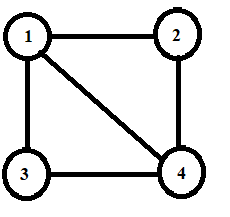
\includegraphics{figures/T4-1.png}
	\caption{a VCLP exact non-bipartite graph}
	\end{minipage}
	\begin{minipage}[t]{0.48\textwidth}
	\centering
	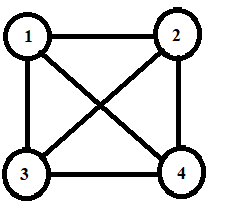
\includegraphics{figures/T4-2.png}
	\caption{a MLP exact but not VCLP exact graph}
	\end{minipage}
	\end{figure}

		1. $G_1$ in figure 1 is not a bipartite graph. $\tau(G_1)=2$, while $\tau(G_1)\geq \tau_{f}(G_1)=(y_1+y_2)+(y_3+y_4)\geq 2$, so $G_1$ is still VCLP exact.
		
		2. For $G_2$ in figure 2, $\tau(G_2)=3$,  $\nu(G_2)=2$, and $\nu_{f}(G_2)=\tau_{f}(G_2)=2\ (y_1=y_2=y_3=y_4=0.5)$. 
		Therefore $\nu(G_2)=\nu_f(G_2)$ and $\tau(G_2)<\tau_f(G_2)$, $G_2$ is MLP exact but not VCLP exact.
		
		3.Define $y$ as follows:$y_u=0$ for $u\in V/Y$, $y_v=\sum\x_e$ for $v\in Y$ and $e=(u,v)$.
		If $\exists e\subseteq Y\ x_e>0$, then $x_e$ is added twice in $|y|$,so $|y|>|x|$.
		And because $x$ is an optimal solution of $\operatorname{MLP}(G)$ and $G$ is VCLP exact, $|x|=\nu_{f}(G)=\tau_{f}(G)=\tau(G)$
		It means among $|Y|=\tau(G)$ vertices there's at least 1 vertex with $y_{v'}>1$, implies that $\sum\x_e>1$ for $e=(u,v')$, which is a contradiction.
		
		4. $V$ can be divided to $Y$ and $V/Y$. 
		For subset $A\subset Y$, denote$B\subset V/Y$ as the neighbour of $A$.
		If $|B|<|A|$, because for $u\in a$,$y_u=1$, changing $y_u$ to $1-\epsilon(0<\epsilon<0.5)$ for $u\in A$and $y_v$ to $\epsilon$ for $v\in B$. $V$ after changing still satisfies $y_u+y_v\geq 1$ and is a smaller solution of VCLP,which is a contradiction.
		 
		So $Y$ and $V/Y$ is a bipartite graph ignoring edges in $Y$ and $V/Y$, and applying Hall's theorem we find a matching of size $|Y|$. 
		Because $\nu(G)\geq|Y|=\tau(G)$ and $\nu(G) \leq \nu_{f}(G)=\tau_{f}(G) \leq \tau(G)$, then we have $\nu(G)=\nu_f(G)$. 
		So $G$ is MLP exact.
		 
	
\end{problem}
\end{document}